%%%%% START PREAMBLE HEADER %%%%%

%%% START REQUIRED PACKAGES %%%

\documentclass[twocolumn]{article}
\usepackage[a4paper, total={7.25in, 9.5in}]{geometry} 
\usepackage{multirow}
\usepackage{multicol}
\usepackage{lipsum}
\usepackage{hyperref}
\usepackage{listings}
\usepackage{graphicx}
\usepackage{import}
\usepackage[table,xcdraw]{xcolor}
\usepackage[export]{adjustbox}
%\usepackage[superscript,biblabel]{cite}
\usepackage{amsmath}
\hypersetup{colorlinks=true,linkcolor=blue,filecolor=magenta,urlcolor=cyan,citecolor=blue}

%%% END REQUIRED PACKAGES %%%                


%%% START NEW COMMANDS new (shortcut) %%%

% This is a paragraph with normal font
\newcommand{\np}[1]{\paragraph*{\normalfont{#1}}}
% This is a text with a color
\newcommand{\ct}[2]{\textcolor{#1}{#2}}
% This is a bold text 
\newcommand{\bt}[1]{\textbf{#1}}
% This is an italic text 
\newcommand{\et}[1]{\emph{#1}}
% This is an underline text 
\newcommand{\ut}[1]{\underline{#1}}
% This is a newline shortcut
\newcommand{\n}{\\}
% This is a numbered equation with break line shortcut
\newcommand{\necbreak}[1]{\begin{equation}\begin{aligned}#1\end{aligned}\end{equation}}
% This is a numbered equation with break line shortcut
\newcommand{\nec}[1]{\begin{equation}#1\end{equation}}
% This is an equation shortcut
\newcommand{\ec}[1]{\begin{center} $#1$ \end{center}}
% Table title with bold text and correct space%
\newcommand{\titleTable}[2]{\np{\bt{Table #1} #2}}% Graph title with bold text and correct space%
\newcommand{\titleGraph}[2]{\np{\bt{Graph #1} #2}}
% Table body with border %
\newcommand{\bodyTable}[2]{\begin{center} \begin{tabular}{|#1|} \hline #2 \hline \end{tabular} \end{center} }
%%% END NEW COMMANDS (shortcuts) %%%


%%% START TITLE SETTINGS %%%
\title{\bt{Decomposition of hydrogen peroxide in the gas phase}}
\author{Pérez Alvarado Luis Raymundo, School of Chemistry, UNAM}
\date{10/02/2021}
%%% END TITLE SETTINGS %%%

%%%%% END PREAMBLE HEADER %%%%%

%%%%%%%%%%%%%%%% START DOCUMENT %%%%%%%%%%%%%%%%
\begin{document}

    %%% THIS CONTENT IS IN ONE COLUMN (START) %%%
    \twocolumn[
        \begin{@twocolumnfalse}

            %% CREATE A TITLE (START) %%
            \maketitle
            %% CREATE A TITLE (END) %%

            %% CREATE A ABSTRACT (START,MAX 250 CHARACTERS) %%
            \begin{abstract}
                \item This report shows the results obtained from modeling the decomposition of $H_2O_2$ in the gas phase with a readical mechanism which was carried out with the $m062x$ method and the base $6-31+(d,p)$ with the $gaussian$ program, the profiles were obtained Of the proposed reactions and the rate constants were calculated, these had errors less than $3kcal/mol$ when compared with the experimental values.
                \item \bt{Keywords:}\em{ radical reaction, transition state, reaction profile, rate constant.}
            \end{abstract}
            %% CREATE A ABSTRACT (END) %%
    
        \end{@twocolumnfalse}
    ]
    %%% THIS CONTENT IS IN ONE COLUMN (END) %%%

    %%% THIS CONTENT IS IN TWO COLUMN (START) %%%


    % SECTION TITLE %
    \section*{Study system \small{$^{\cite{art:descomposition}\cite{web:rad}}$} }

    \np{The global reaction of descomposition of $H_2O_2$ is show in \eqref{1}.}

    \nec{2H_2O_2 \rightarrow 2H_2O + O_2 \label{1}}

    \np{The reaction by radical are made in four steps show in \eqref{2}, \eqref{3}, \eqref{4} and \eqref{5} with his correspond stequeometry.}

    \nec{H_2O_2 \rightarrow 2HO\cdot ~(initiation)\label{2}}

    \nec{HO\cdot + H_2O_2 \rightarrow HO_2\cdot + H_2O ~(propagation
    ) \label{3}}

    \nec{HO_2\cdot + HO_2\cdot \rightarrow O_2 + H_2O_2 ~(termination
    )\label{4}}

    \nec{HO_2\cdot + HO\cdot \rightarrow O_2 + H_2O ~(termination
    )\label{5}}

    \np{The sum of equation 2 to 5 give \eqref{1} }

    \section*{Objectives}

    \np{Model the decomposition of hydrogen peroxide in gas phase, propose and find the transition state (TS) of each reaction and build a profile reaction with his potential energies, also calculate the rate constant for each of them, and compare with literature values.}

    \section*{Materials and methods}

    \np{The modeling of the systems $H_2O_2$,$H_2O$,$O_2$,$HO_2\cdot$,  $HO\cdot$ and transition states were performed with gaussView.}

    \np{Calculations were done with a laptop with an i7-8750H processor with 8GB of RAM with gaussian09W.}

    % START FIGURE %
    \begin{figure}[h!]
        % Reactive %
        \centering
        \begin{minipage}[b]{0.49\textwidth}
            \centering
          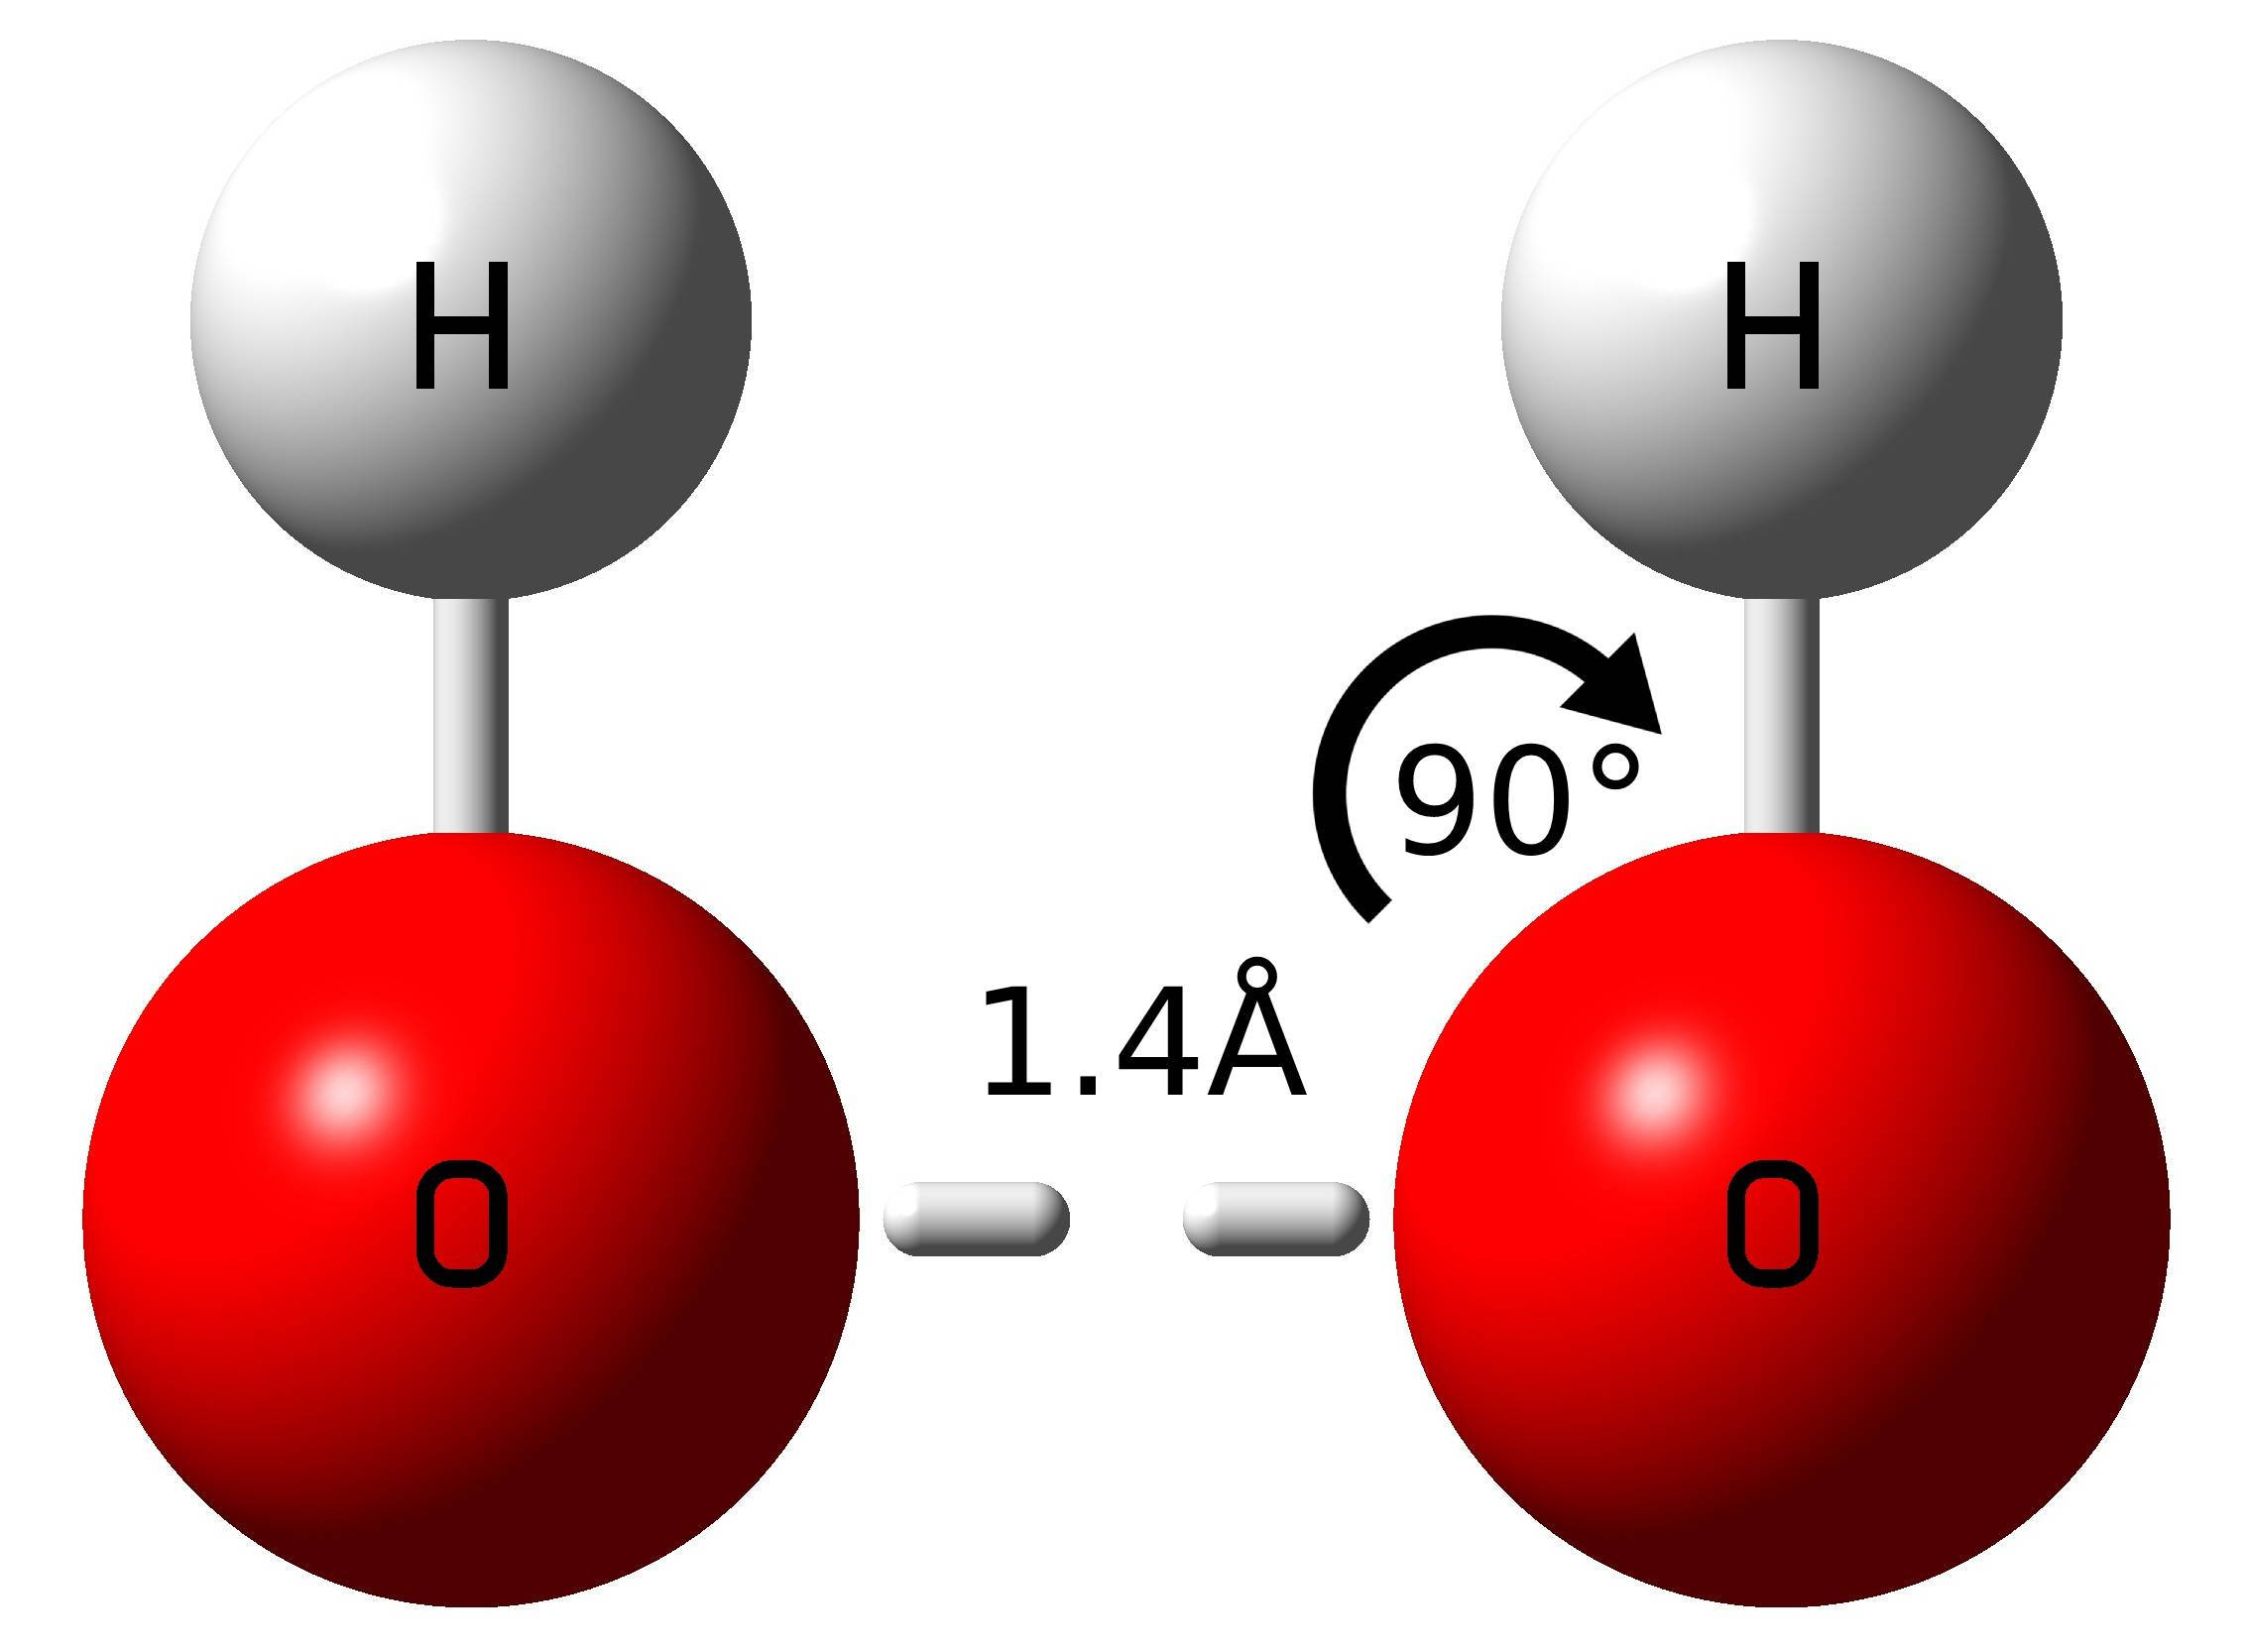
\includegraphics[scale=0.085]{s1.jpg}
          \caption{TS1.}
        \end{minipage}
        \centering
        \begin{minipage}[b]{0.49\textwidth}
            \centering
          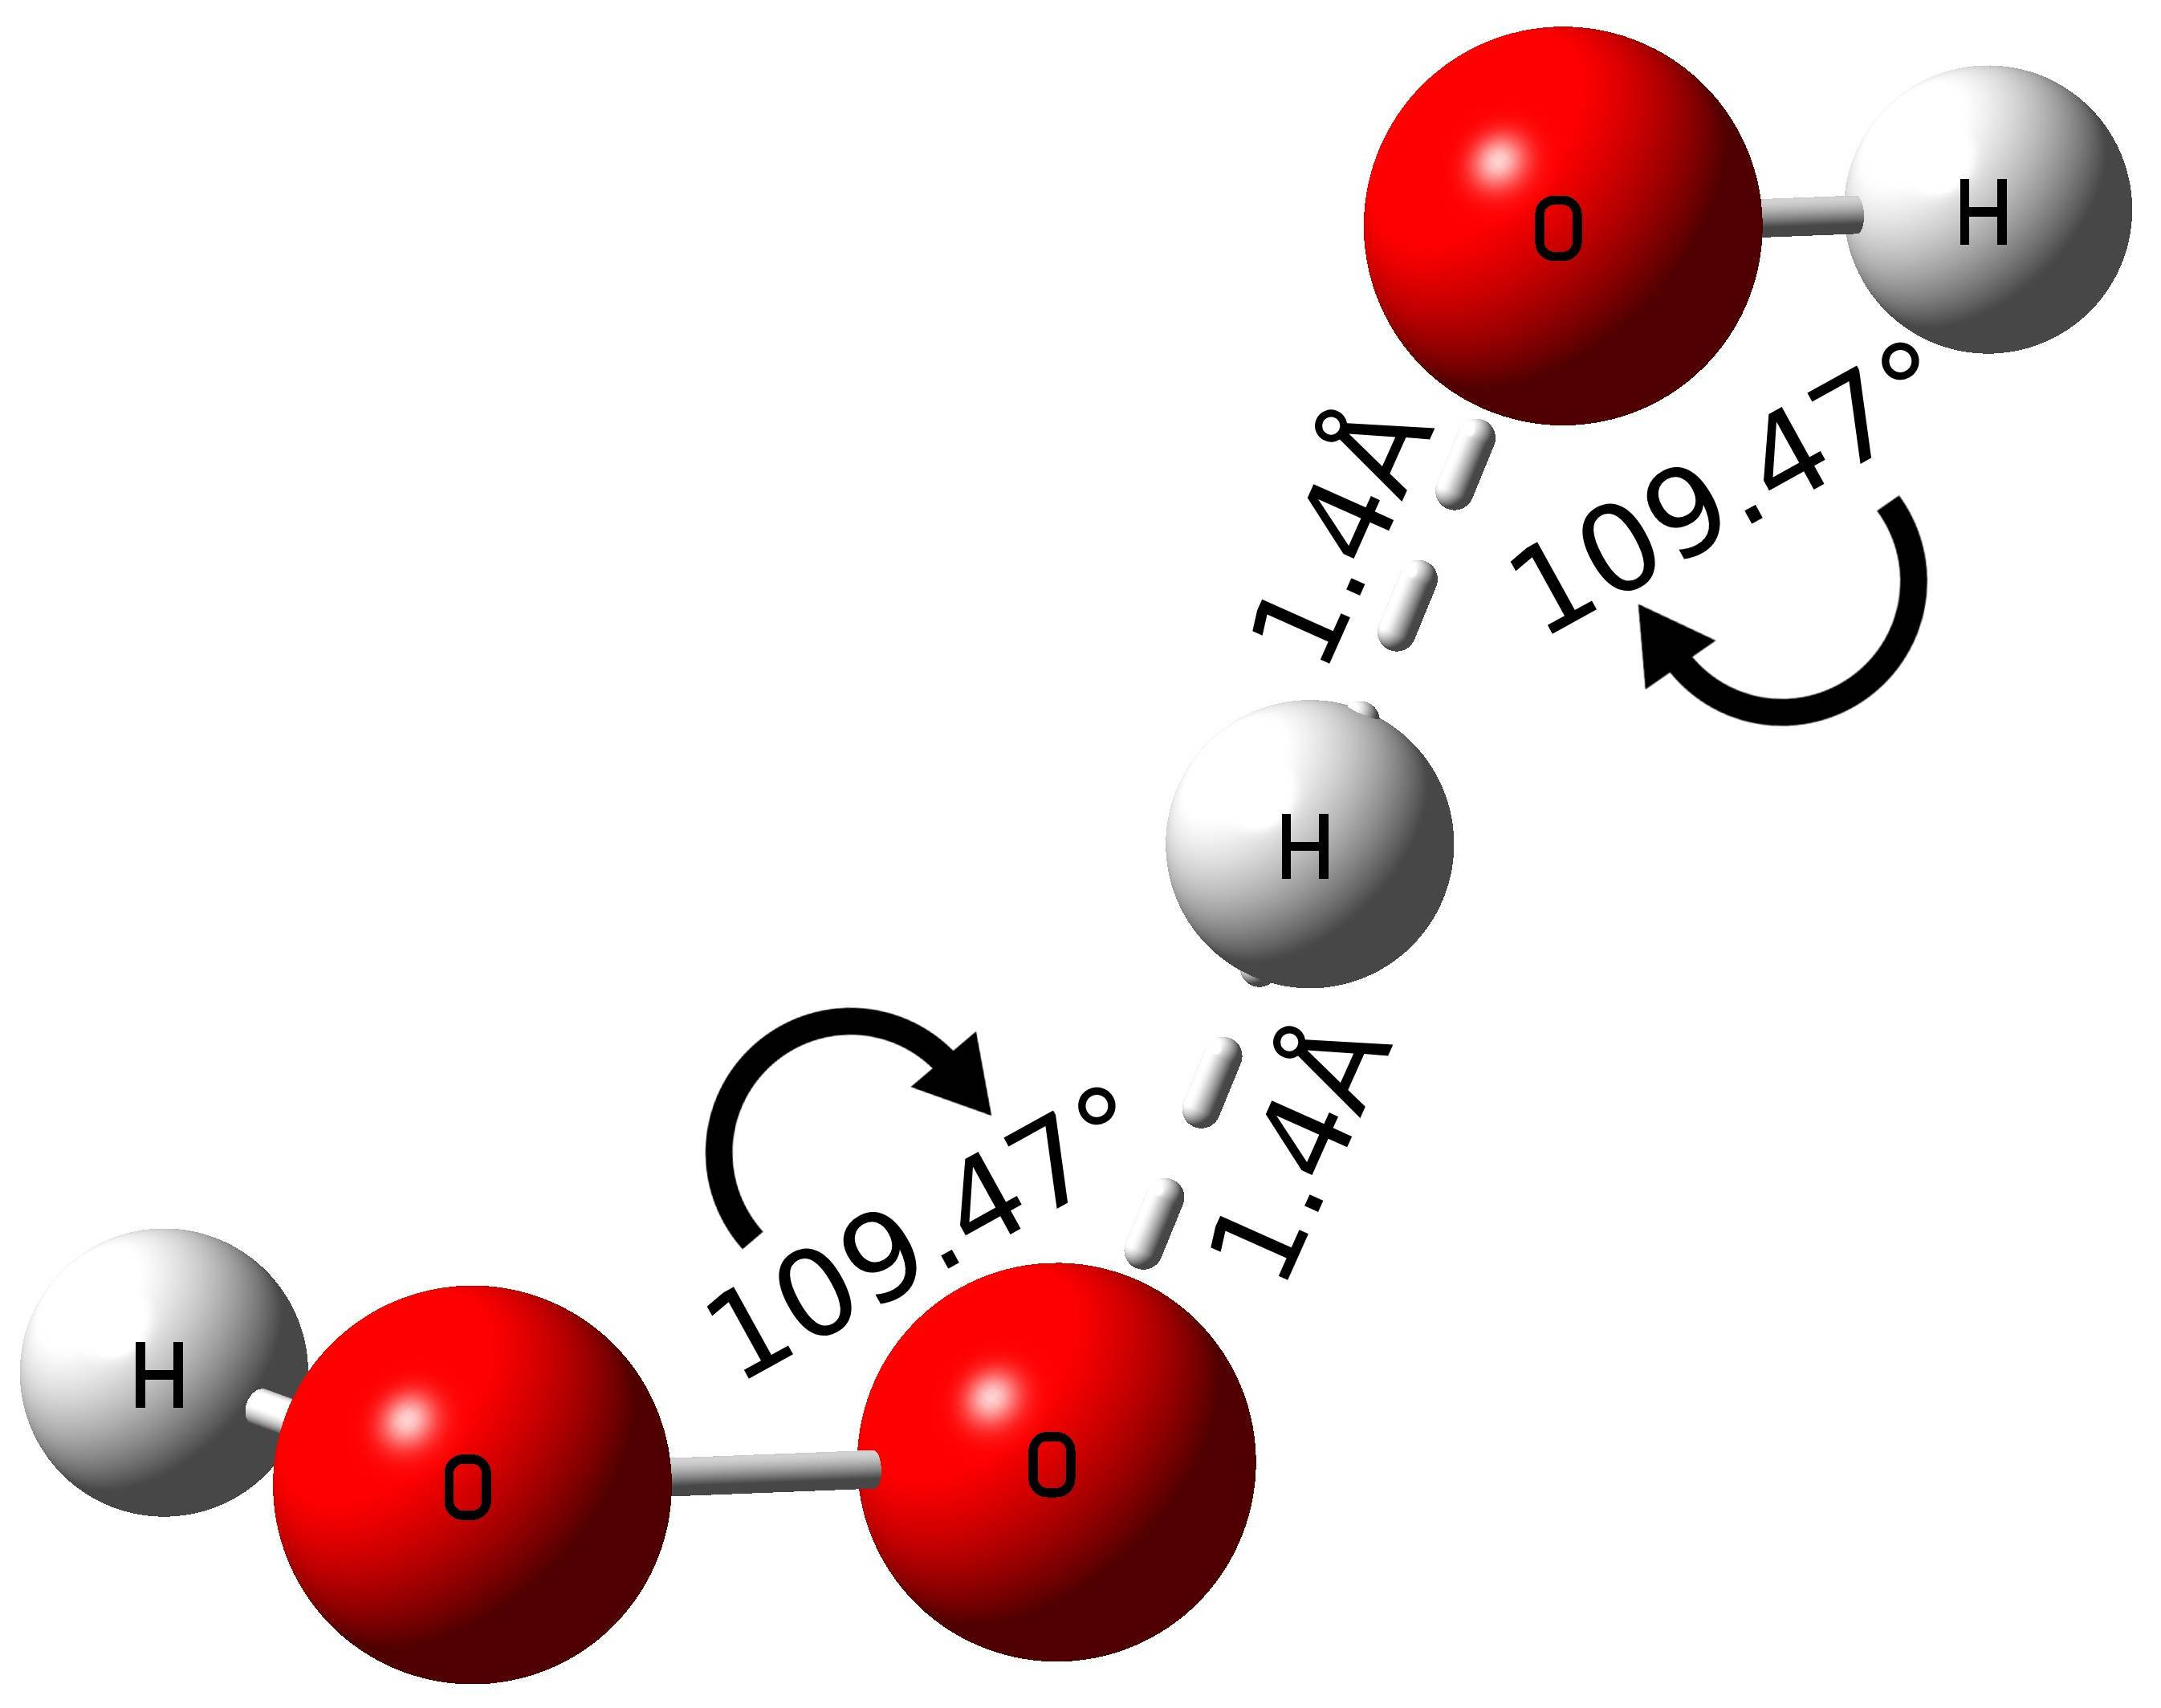
\includegraphics[scale=0.13]{s2.jpg}
          \caption{TS2.}
        \end{minipage}
        \begin{minipage}[b]{0.49\textwidth}
            \centering
          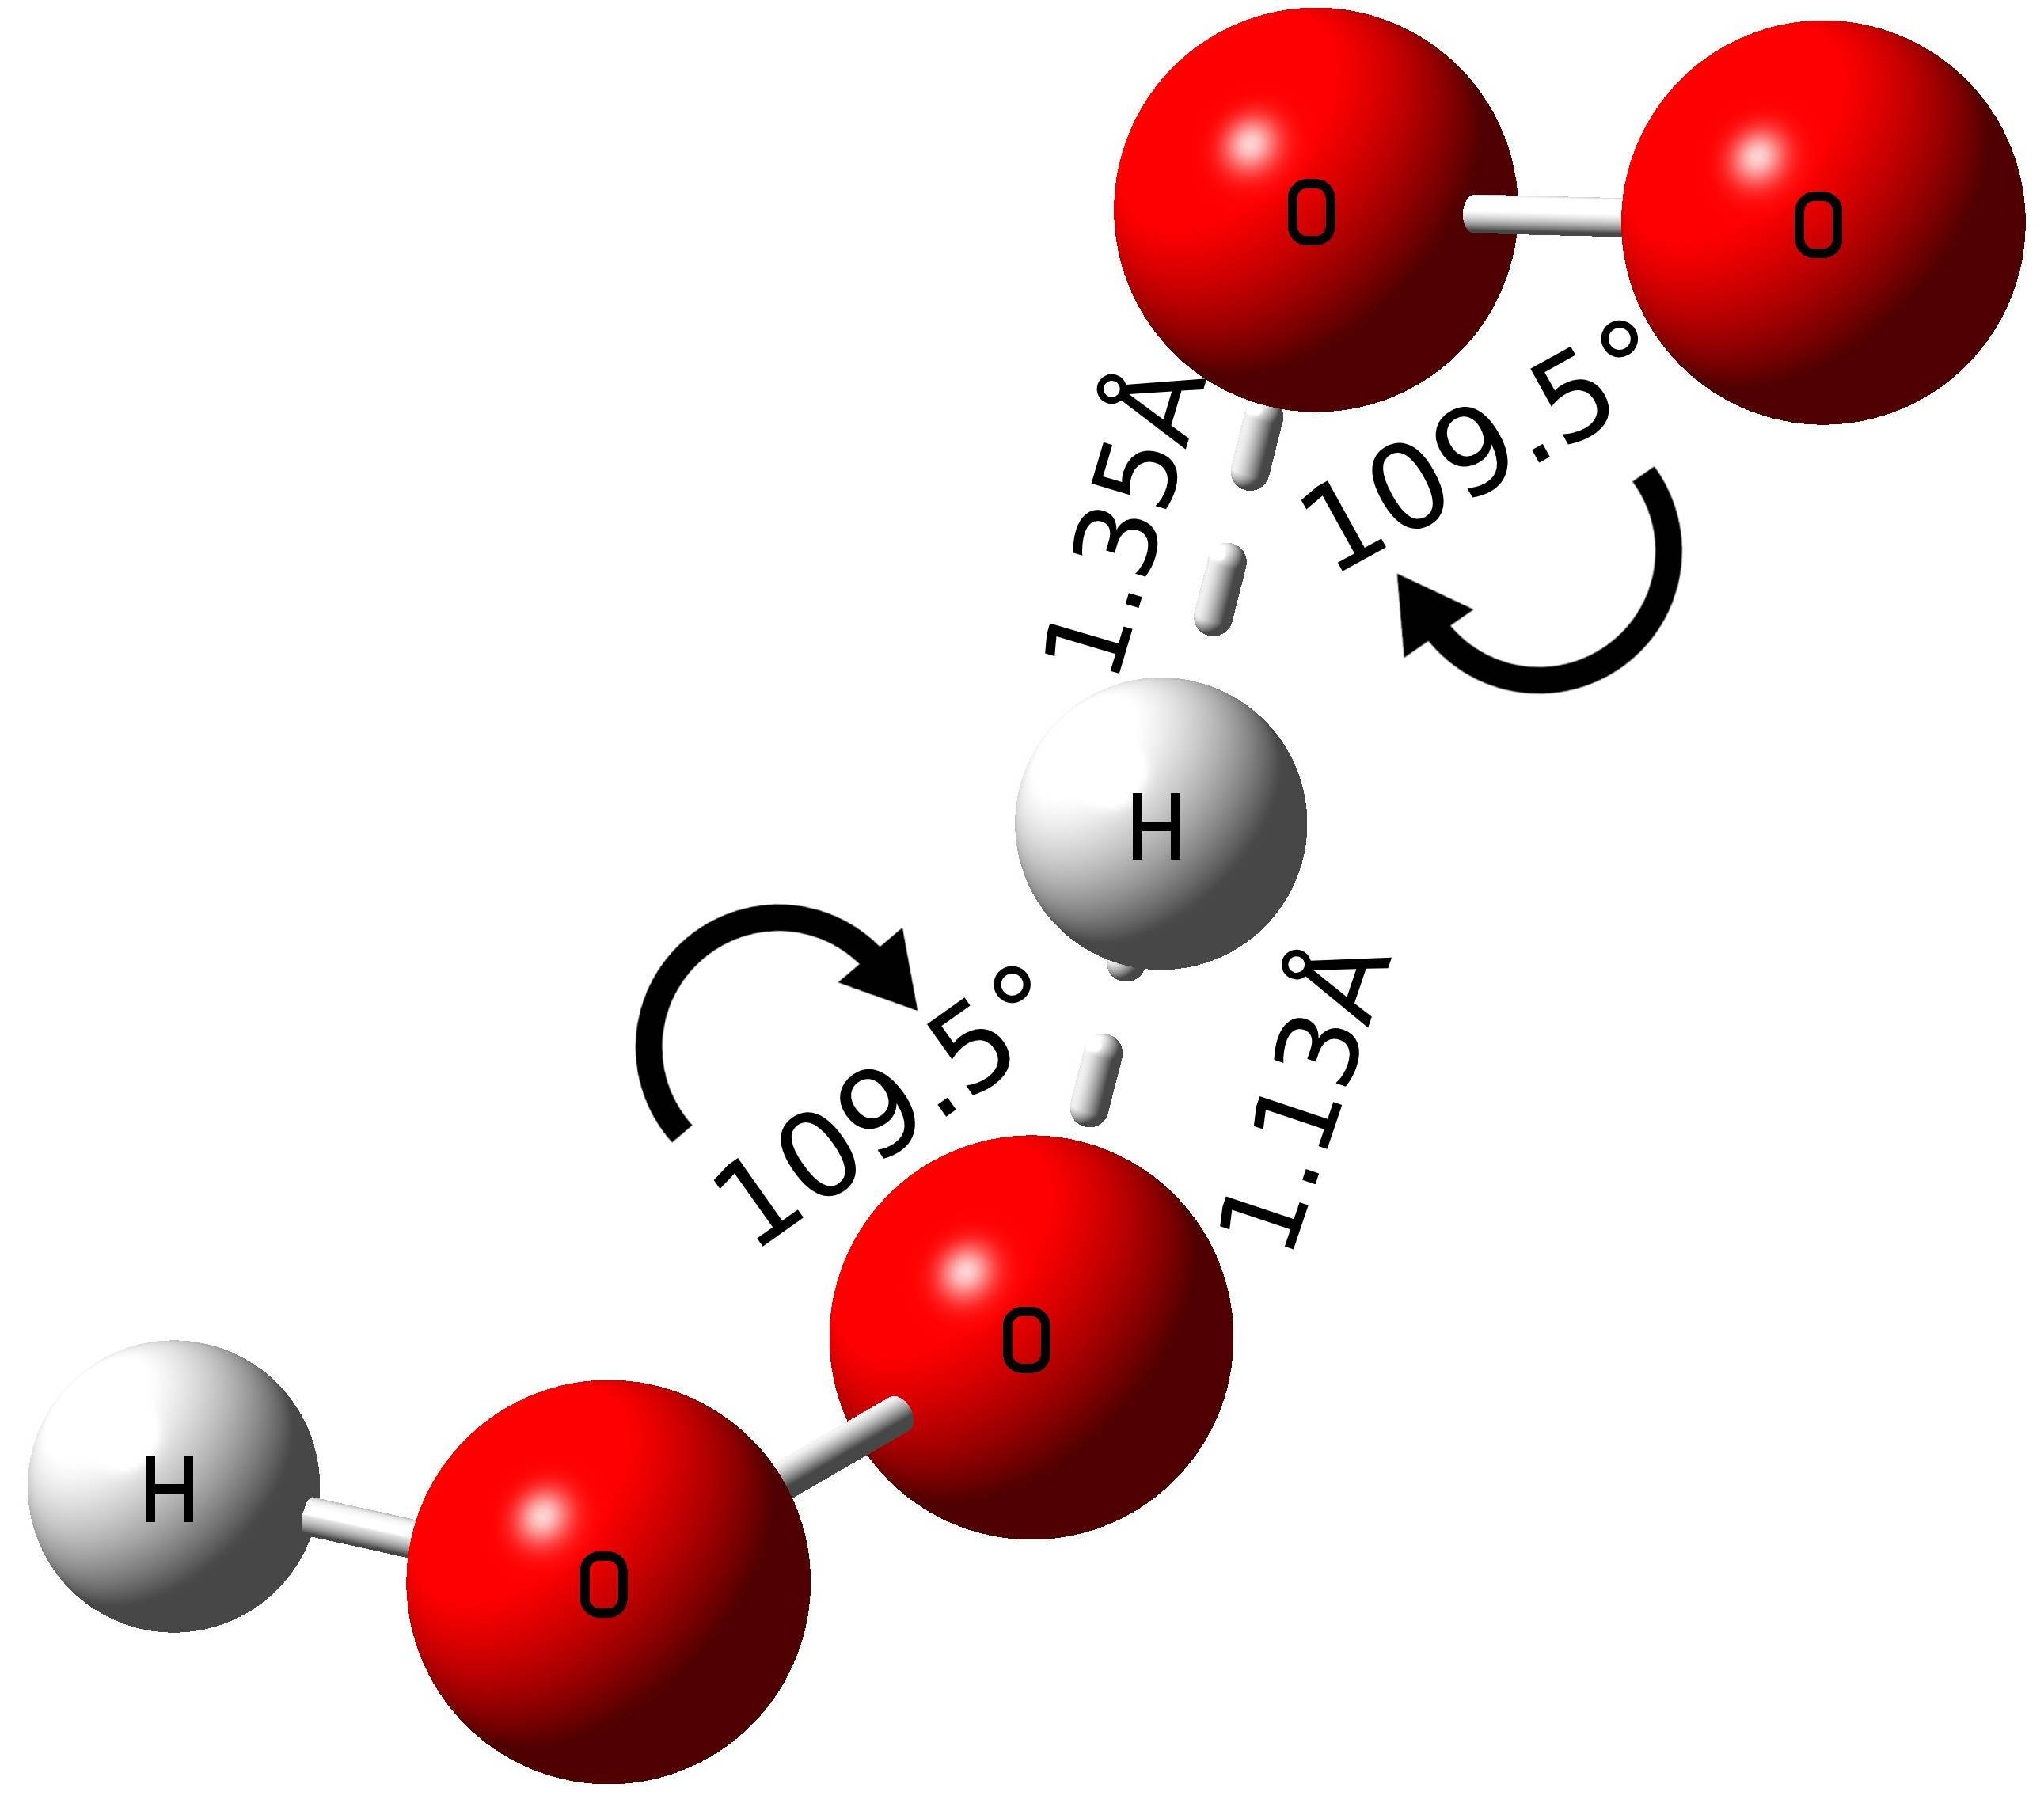
\includegraphics[scale=0.13]{s3.jpg}
          \caption{TS3.}
        \end{minipage}
        
        %water%
       
    \end{figure}
    % END FIGURE %

    \begin{figure}[h!]
        % Reactive %
        \centering
        
        \begin{minipage}[b]{0.49\textwidth}
            \centering
        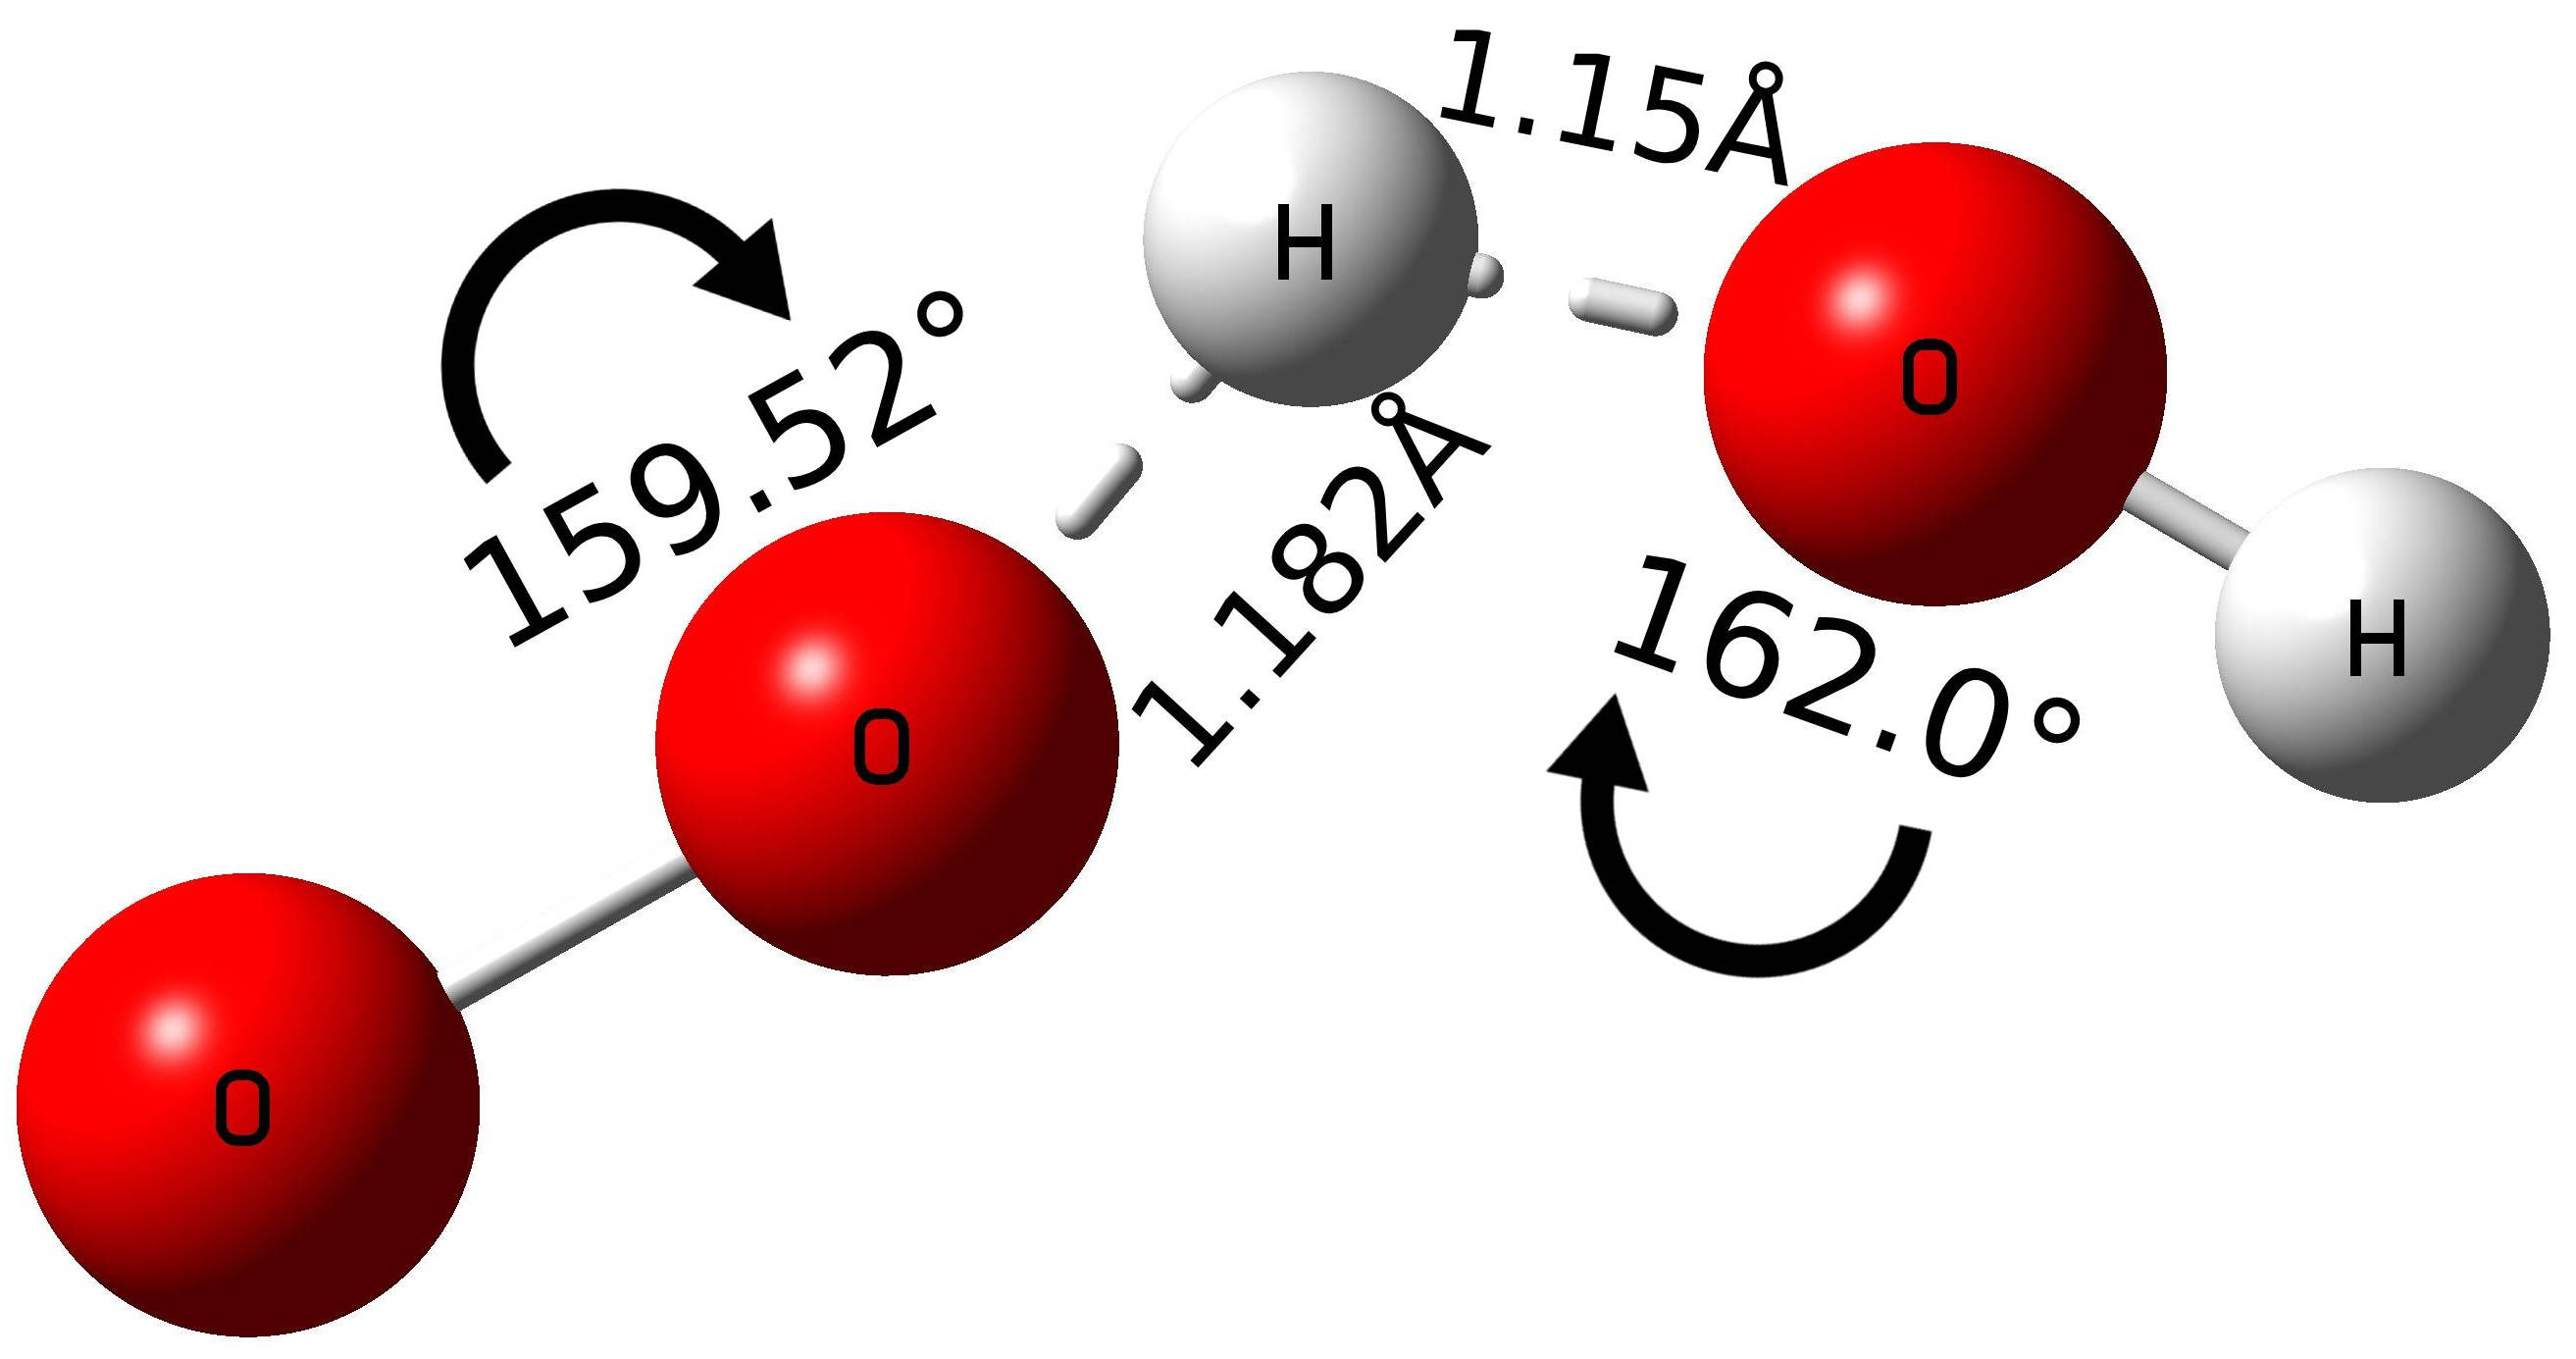
\includegraphics[scale=0.145]{s4.jpg}
        \caption{TS4.}
        \end{minipage}

    \end{figure}

    \np{The reactants and products were run with the following settings.\n}

    \begin{lstlisting}[frame=single,gobble=10] 
        ~ % nprocshared=4
        ~ % mem=1500MB
        ~ # opt freq=noraman 6-31+g(d,p) M062X 
    \end{lstlisting}

    \np{The transition states (figures 1-4) were run with the following settings.\n}

    \begin{lstlisting}[frame=single,gobble=10] 
        ~ % nprocshared=4
        ~ % mem=1500MB
        ~ # opt(calcfc,ts,noeigen,maxcycles=100) 
        ~   freq=noraman 6-31+g(d,p) M062X 
    \end{lstlisting}

    \np{\bt{NOTE:} The transition state configuration shown is the initial configuration before the run, and those configurations were found after multiples test with other configurations where they varied bond distances and angles.}

    \section*{Results}

    \np{The values of H and G obtained from the calculations are shown in table 1.}

    \titleTable{1}{Calculated values of H and G.}

    \begin{center}
        \item \import{./}{table1.tex}
    \end{center}
    

    \np{The values of G and H were processed in table 2 (see appendix) to calculate $\Delta G$ and $\Delta H$ to build the reaction profiles, and table 3 shows the speed constants obtained.}

    \titleGraph{1}{Reaction profiles of free energy.}

    \begin{center}
        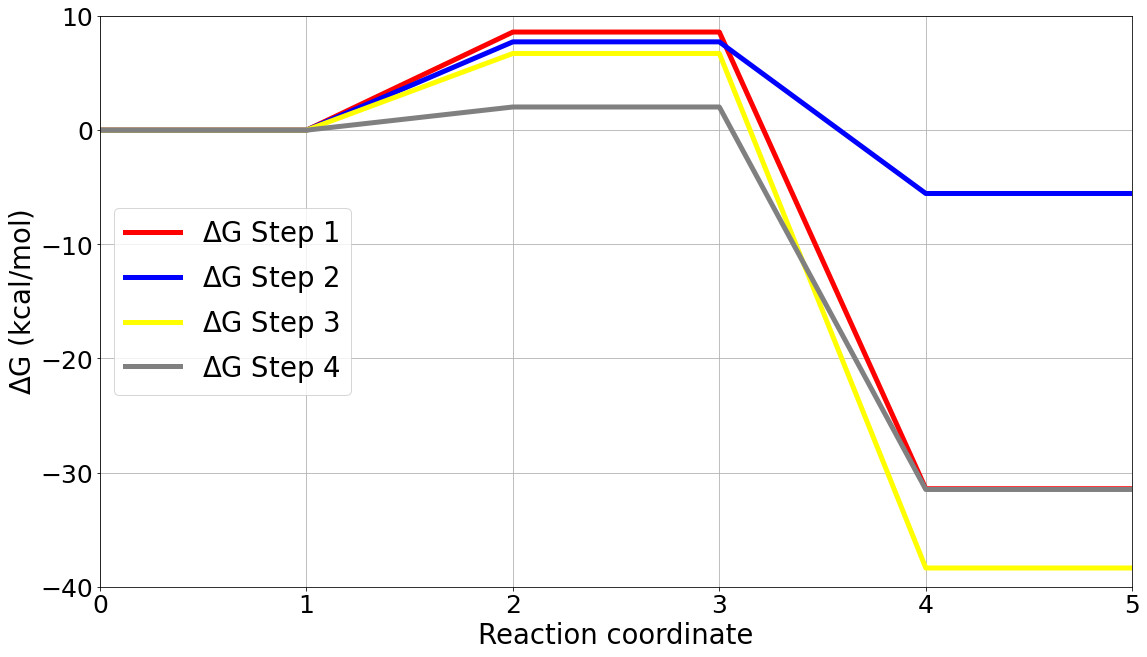
\includegraphics[scale=0.22]{g.jpg}
    \end{center}

    \titleGraph{2}{Reaction profiles of enthalpy.}

    \begin{center}
        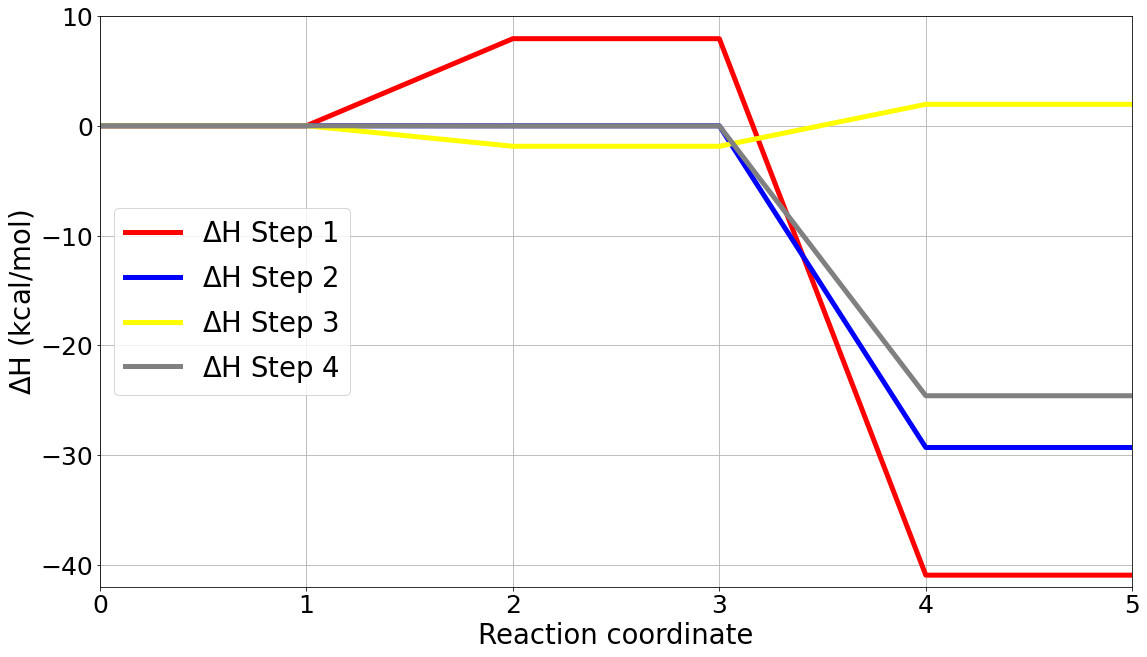
\includegraphics[scale=0.22]{h.jpg}
    \end{center}

    \titleGraph{3}{Reaction profiles of $\Delta G$ and $\Delta H$.}

    \begin{center}
        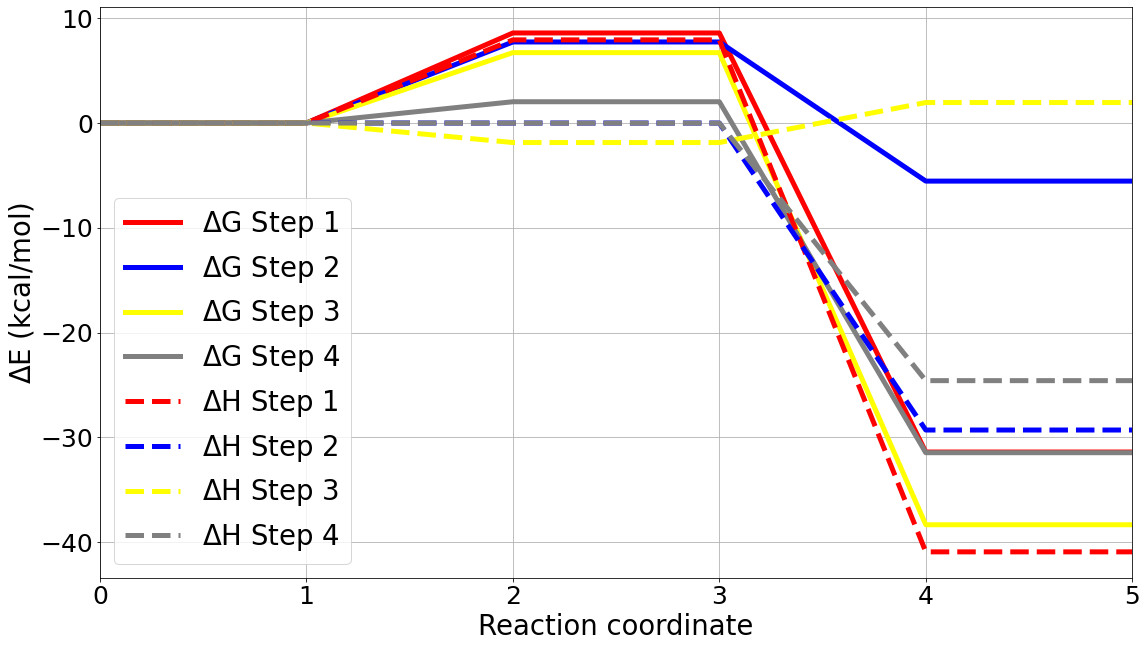
\includegraphics[scale=0.22]{E.jpg}
    \end{center}

    \titleTable{3}{Rate contant calculated and comparation with the experimental values.}

    \begin{center}
        \item \import{./}{table3.tex}
    \end{center}

    \np{~}

    \section*{Discussion}

    \np{The free energy reaction profile shows that all the steps are exergonic, highlighting that the most exergonic is step \eqref{4} and the least exergonic is step \eqref{3}, it should be noted that step \eqref{2} is the step that has the highest activation energy of all the steps which makes sense since the OO bond is broken and step \eqref{5} is the one that requires the least free energy.}

    \np{In the case of graph 2, the fact that breaking the link requires a large amount of energy is much more marked, except for step \eqref{4} all the other steps are exergonic, despite the fact that step \eqref{4} its activation enthalpy is negative free energy is not, so we can denote the importance of the entropy contribution, this can be seen much better in graph 3 where the free energy and entlapy are plotted.}

    \np{The calculations of the speed constants were carried out using the configurations shown in figures 1-4 for the calculations of the transition states, in table 3 it can be seen that the comparison of the calculated speed constants with the experimental ones are compared in two ways in which you can see if the calculated constant is faster (column 3) or slower (column 4).}

    \np{Step 1 and 3 are slower than the experimental step one by $\approx$ 6 times and the third $\approx$ 3 in step 2 and 4 both are faster the second $\approx$ 1.5 times faster and in the fourth step it is $\approx$ 95 times, with the exception of the fourth step, the calculated constants present values very close to the experimental ones, so we could say that the calculated configurations are very close to reality, in the case of the fourth step this has an error less than $3kcal/mol$,despite if it is not very good it is an acceptable value.}

    \np{The values obtained from the velocity constants are directly related to the activation energy $\Delta G^{\ddagger}$ obtained, more specifically from the free energy $G$ calculated from the transition state, so the proper configuration for the transition state is of great importance for the calculations of constant speed and construction of reaction profiles, which may seem like an easy task, but it is a great job to get a suitable configuration and even closer to the reality of the experiment.}

    \np{As perspectives of this study, it could be used as a basis for the study of the same reaction with conditions closer to the experimental ones, this is to perform the calculation at high temperatures, which is when thermal decomposition is carried out, at low pressures or nitrogen atmospheres, or a solvent such as water or another, or the same process but catalyzed by means of some catalyst.}

    \np{As conclusions it was possible to propose the reaction mechanism for the decomposition of hydrogen peroxide in the gas phase by the radical pathway proposed ref, the reaction profiles were constructed and analyzed and the rate constants were calculated, which were close to the experimental ones, which which confirmed that the transition states are good approximations, this despite being a very small study, shows us the potential that computational chemistry has to model reactions.}


    % DEFINE STYLE FORMAT%
    \bibliographystyle{ieeetr}
    % SPECIFY THE FILE NAMEw %
    \bibliography{references}

    %START APPENDIX (always in last page)%
    \appendix
    % CHANGE FROM X COLUMN TO ANOTHER COLUMNS EJ 2 -> 1%
    \onecolumn
    \section{Appendix}
    \begin{center}
      \item \titleTable{2}{Calculation $pk_a$ with method 1.}
      \item \import{./}{table2.tex}
    \end{center}

    
  

    %% END REFERENCES %% 

    %%% THIS CONTENT IS IN TWO COLUMN (END) %%%

\end{document}
%%%%%%%%%%%%%%%% END DOCUMENT %%%%%%%%%%%%%%%%